%%%%%%%%%%%%%%%%%%%%%%%%%%%%%%%%%%%%%%%%
% Class options                        %
%%%%%%%%%%%%%%%%%%%%%%%%%%%%%%%%%%%%%%%%
% Orientation:                         %
% portrait (default), landscape        %
%                                      %
% Paper size:                          %
% a0paper (default), a1paper, a2paper, %
% a3paper, a4paper, a5paper, a6paper   %
%                                      %
% Language:                            %
% english (default), norsk             %
%%%%%%%%%%%%%%%%%%%%%%%%%%%%%%%%%%%%%%%%
\documentclass{psuposter}


\usepackage{natbib}
\usepackage{lipsum}                                % Dummy text
\usepackage[figwidth = 0.98\linewidth]{todonotes}  % Dummy image (and more!)
\usepackage[absolute, overlay]{textpos}            % Figure placement
\setlength{\TPHorizModule}{\paperwidth}
\setlength{\TPVertModule}{\paperheight}

\setcitestyle{numbers,square}


\title{Some Lengthy and Technical Title}
\author
{%
    Speaker Name\inst{1}
}
%% Optional:
\institute
{
    \inst{1} University of Speaker, Department of Speaker
}
% Or:
%\institute{Contact information}


%% Remove footline:
%\setbeamertemplate{footline}{}


\begin{document}
\begin{frame}
\begin{columns}[onlytextwidth]


\begin{column}{0.5\textwidth - 1.5cm}
    \begin{block}{Speaker Biographic Summary}
    	\begin{center}
	    	
\includegraphics[width=0.6\textwidth]{psuposter-images/lion}    		
    	\end{center}
        This paragraph represents the speaker bio. Include their name, affiliation (yes it is included above too..). Also describe their educational background briefly, as well as research interests. If they have won any notable awards / etc, try to mention that as well.
    \end{block}
%
%    \begin{exampleblock}{Does it come in black?}
%        Sure, use an \textbf{exampleblock}!
%    \end{exampleblock}
%
%    \begin{alertblock}{How do you make it pop?}
%        Use an \alert{alertblock}!
%    \end{alertblock}
%
%    \begin{block}{Method}
%        \lipsum[1]
%    \end{block}

    \begin{block}{Research Interests}
        \lipsum[2]
        \begin{center}
	    	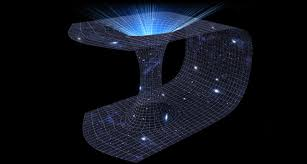
\includegraphics[width=0.6\textwidth]{psuposter-images/sample-research}    		
    	\end{center}
    \end{block}
\end{column}


\begin{column}{0.5\textwidth - 1.5cm}
    \begin{block}{Talk Abstract}
        \lipsum[4]
    \end{block}

    \begin{block}{Brief Background}
        \lipsum[2]
        \cite{ashtekarLoopQuantumGravity2017}
%        \lipsum[3]
        $$\int_{\partial \Omega} \omega = \int_{\Omega} d \omega$$
        \lipsum[2]
        \cite{anselmiPredictionsQuantumGravity2020}
    \end{block}

    \begin{block}{References}
%        \lipsum[1]
        \bibliographystyle{aipnum4-1}
		\bibliography{references}
    \end{block}

%    \begin{block}{Contact information}
%        \lipsum[75]
%    \end{block}
\end{column}


\end{columns}


\begin{textblock}{0.5}(0.18, 0.94)
    \color{white}
    \sffamily
    \textbf{Eberly College of Science}
    \\
    Department of Physics
    
\end{textblock}


\end{frame}
\end{document}